\begin{solution}{normal}
Note that in the dual circuit drawn, all resistors have a resistance one quarter of that of a corresponding resistor in the original circuit.
\begin{center}
    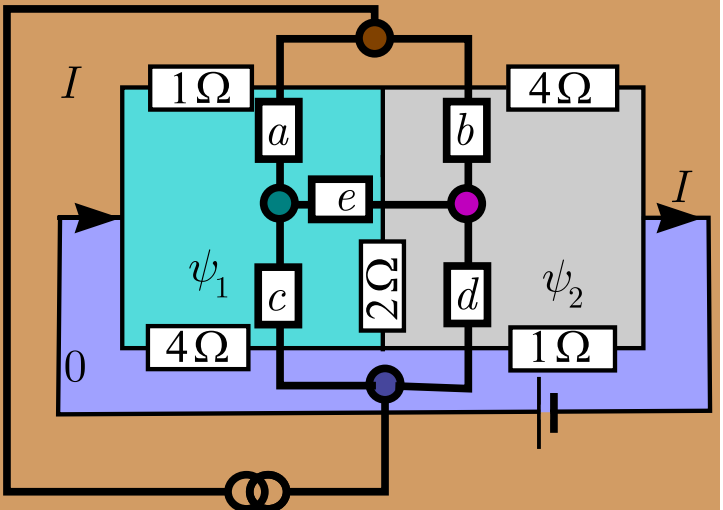
\includegraphics[width=0.6\linewidth]{Figures/pr15_sol.PNG}
\end{center}
For example, we have $a=d=1\,\Omega$, $c=b=0.25\,\Omega$, and $e=0.5\,\Omega$. These are obtained by letting the conductance of the original resistor elements the circuit passes through be the resistance of the dual resistors. Here, $a$ and $d$ correspond to one fourth of the $4\,\Omega$ resistors, $b$ and $c$ correspond to one fourth of the $1\,\Omega$ resistors and $e$ corresponds to one fourth of the $2\,\Omega resistors$. Therefore, we can say that:
$$R^* = \frac{R}{4}$$
where $R^*$ is the effective resistance of the dual circuit and $R$ is the effective resistance of the original circuit. However, from the stream function method, we must also have:
$$R^* = \frac{1}{R}$$
so we get:
$$\frac{R}{4}=\frac{1}{R} \implies \boxed{R=2\,\Omega}$$
\end{solution}